\documentclass[english, 12pt]{article}

\usepackage{amsmath}
\usepackage{amssymb}
\usepackage[style=vancouver, sorting=none, doi=true, urldate=iso, seconds=true]{biblatex}
\usepackage{float}
\usepackage{hyperref}
\usepackage{tkz-euclide}

\usetikzlibrary{arrows.meta, decorations.markings}
\abovecaptionskip=3pt
\parindent=0pt
\parskip=8.0pt
\baselineskip=12pt
\oddsidemargin=-0.5cm
\textwidth=17cm
\topmargin=-1.4cm
\textheight=23.0cm

\addbibresource{references.bib}

\title{MTH3022 Project (TODO: Name?)}
\author{} % TODO: Should fill in
\date{}

\begin{document}

\maketitle

\section{Semantic Web}
The semantic web is a set of standards defined by the World Wide Web Consortium\cite{w3c_website} with the goal of allowing computers to parse and understand internet data. The primary technologies they developed for this are the Resource Description Framework\cite{w3c_rdf} (RDF) and the Web Ontology Language\cite{w3c_owl} (OWL).

\subsection{RDF}
The Resource Description Framework is designed to standardise links between subjects and objects, and while it was initially designed for metadata, it is now used generally across a wide variety of domains. At its core are RDF graphs, sets of \texttt{(subject, predicate, object)} triples. \texttt{subject}s and \texttt{object}s are called resources (typically either text or IRIs\cite{iri_rfc}) and denote something that exists, while \texttt{predicates} denote properties and are always IRIs. These depict a relationship between the \texttt{subject} and the \texttt{object}, with \texttt{predicate} indicating the type of relationship. This can be depicted as a directed graph, with \texttt{subject}s and \texttt{object}s being vertices, and \texttt{predicate}s being edge labels. For example the RDF graph \{\texttt{(sky, colour, blue), (sky, above, grass), (sky, above, trees), (grass, colour, green), (trees, colour, green)}\} could be depicted as below.
\begin{figure}[H]
\centering
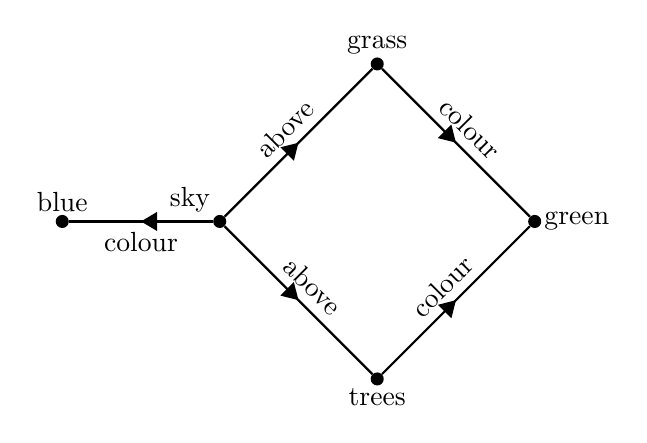
\begin{tikzpicture}
\tkzLabelPoint[above left](0, -2){sky}
\node[circle, fill=black, scale=0.5] at (0, -2) (sky) {};
\tkzLabelPoint[above](2, 0){grass}
\node[circle, fill=black, scale=0.5] at (2, 0) (grass) {};
\tkzLabelPoint[below](2, -4){trees}
\node[circle, fill=black, scale=0.5] at (2, -4) (trees) {};
\tkzLabelPoint[right](4, -2){green}
\node[circle, fill=black, scale=0.5] at (4, -2) (green) {};
\tkzLabelPoint[above](-2, -2){blue}
\node[circle, fill=black, scale=0.5] at (-2, -2) (blue) {};

\begin{scope}[thick,decoration={markings, mark=at position 0.5 with {\arrow{Triangle[scale=1.2]}}}]
\draw[postaction={decorate}] (sky) -- (blue) node[midway, below, sloped]{colour};
\draw[postaction={decorate}] (sky) -- (grass) node[midway, above, sloped]{above};
\draw[postaction={decorate}] (sky) -- (trees) node[midway, above, sloped]{above};
\draw[postaction={decorate}] (grass) -- (green) node[midway, above, sloped]{colour}; 
\draw[postaction={decorate}] (trees) -- (green) node[midway, above, sloped]{colour};
\end{scope}
\end{tikzpicture}
% TODO: Should probably have a caption
\end{figure}

\subsection{OWL}
TODO

\printbibliography

\end{document}
